% ============================================================
%  Healthy Economies, Healthy Communities
%  Mastercard IGS × AUC 2026 Data Science Challenge
%  Jackson State University
% ============================================================
\documentclass[10pt, letterpaper]{article}

% ── Packages ─────────────────────────────────────────────────
\usepackage[margin=1in, top=0.85in, bottom=0.85in]{geometry}
\usepackage[T1]{fontenc}
\usepackage{lmodern}
\usepackage{microtype}
\usepackage{graphicx}
\usepackage{subcaption}
\usepackage{booktabs}
\usepackage{array}
\usepackage{multirow}
\usepackage{amsmath}
\usepackage{xcolor}
\usepackage{enumitem}
\usepackage{fancyhdr}
\usepackage{titlesec}
\usepackage{abstract}
\usepackage{parskip}
\usepackage[hidelinks, colorlinks=true,
            linkcolor=mcblue, citecolor=mcblue, urlcolor=mcblue]{hyperref}

% TikZ
\usepackage{tikz}
\usetikzlibrary{shapes.geometric, arrows.meta, positioning,
                fit, backgrounds, calc}

% ── Colors ───────────────────────────────────────────────────
\definecolor{mcblue}{RGB}{37,  99, 235}
\definecolor{deltared}{RGB}{220, 38,  38}
\definecolor{turngreen}{RGB}{  5,150, 105}
\definecolor{lightgray}{RGB}{248,250,252}
\definecolor{midgray}{RGB}{156,163,175}
\definecolor{darkgray}{RGB}{55, 65,  81}

% ── Typography ────────────────────────────────────────────────
\titleformat{\section}
  {\normalfont\large\bfseries\color{mcblue}}{\thesection}{0.8em}{}
\titleformat{\subsection}
  {\normalfont\normalsize\bfseries\color{darkgray}}{\thesubsection}{0.8em}{}
\titlespacing{\section}{0pt}{14pt plus 2pt minus 2pt}{4pt}
\titlespacing{\subsection}{0pt}{10pt plus 2pt}{3pt}

% ── Header / footer ──────────────────────────────────────────
\pagestyle{fancy}
\fancyhf{}
\renewcommand{\headrulewidth}{0.4pt}
\fancyhead[L]{\small\textcolor{midgray}{Healthy Economies, Healthy Communities}}
\fancyhead[R]{\small\textcolor{midgray}{AUC × Mastercard IGS Challenge 2026}}
\fancyfoot[C]{\small\thepage}

% ── Helpers ──────────────────────────────────────────────────
\newcommand{\igs}{\textsc{igs}}
\newcommand{\shap}{\textsc{shap}}
\setlength{\absleftindent}{0pt}
\setlength{\absrightindent}{0pt}

% ─────────────────────────────────────────────────────────────
\begin{document}
% ─────────────────────────────────────────────────────────────

% ── Title block ──────────────────────────────────────────────
{%
  \centering
  {\fontsize{15}{18}\bfseries\color{mcblue}
    Healthy Economies, Healthy Communities\\[4pt]}
  {\fontsize{11}{14}\bfseries
    What Drives Economic Turnaround in Distressed US Communities?\\
    A Machine-Learning and SHAP Analysis of the Mississippi Delta\\[8pt]}
  {\normalsize
    Jackson State University \quad|\quad
    AUC × Mastercard Inclusive Growth Score Challenge 2026\\[4pt]}
  {\small\textcolor{midgray}{Grand Finale — April 30, 2026}}\\[12pt]
  \rule{\textwidth}{0.4pt}\\[8pt]
}

% ── Abstract ─────────────────────────────────────────────────
\begin{abstract}
\noindent
Among the \textbf{25,142} US census tracts that fell below an Inclusive
Growth Score (\igs{}) of 45 in 2017, only \textbf{34\%} managed to
cross that threshold by 2025.  We train a three-model machine-learning
ensemble—Logistic Regression, Random Forest, and Gradient
Boosting—on 89 granular features drawn from 10 public datasets,
then apply TreeSHAP to identify the precise drivers of
community recovery.  Our central finding is that \textbf{chronic
disease burden} (dental-visit rates, preventive screenings),
\textbf{commercial ecosystem diversity}, and \textbf{broadband
connectivity} are the strongest predictors of turnaround—not aggregate
healthcare counts or composite index scores.  We operationalise these
findings as an \emph{Investment Priority Matrix} that maps every
feature to an actionable quadrant (Act Now / Protect / Second Wave /
Monitor) for each of the nine Mississippi Delta counties.  All data,
models, and an interactive Streamlit dashboard are publicly available.
\end{abstract}

\rule{\textwidth}{0.4pt}
\vspace{6pt}

% ─────────────────────────────────────────────────────────────
\section{Introduction}
% ─────────────────────────────────────────────────────────────

Economic vulnerability is self-reinforcing.  Communities that lack
commercial diversity, broadband access, or adequate preventive
healthcare tend to remain stuck in cycles of low growth, poor health
outcomes, and outmigration.  The \textbf{Mastercard Inclusive Growth
Score} (\igs{}) provides a composite, tract-level measure of economic
inclusion across Place, Community, and Economy pillars, updated
annually.

Figure~\ref{fig:trajectory} makes the central problem concrete: the
nine-county Mississippi Delta has maintained a mean \igs{}
\textasciitilde{}13 points below the national average every year from
2017 to 2025, and has never once crossed the vulnerability threshold
of 45.  Mississippi as a state also lags, but the Delta's gap is
qualitatively different—persistent, deep, and geographically
concentrated.

\begin{figure}[ht]
  \centering
  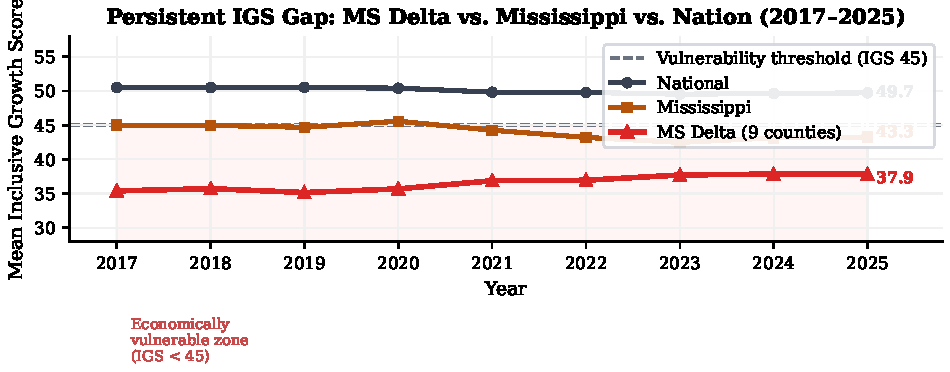
\includegraphics[width=\linewidth]{figures/fig1_igs_trajectory.pdf}
  \caption{Mean Inclusive Growth Score by year for the national
    baseline, Mississippi, and the nine-county MS Delta.  The shaded
    region marks the economically vulnerable zone (IGS $<$ 45).  The
    Delta has remained roughly 13 points below the national mean
    throughout the study period.}
  \label{fig:trajectory}
\end{figure}

The key question this work addresses is: \textbf{among communities
that start below IGS~45, what distinguishes those that escape from
those that remain stuck?}  Answering that question at the feature
level—not the composite-index level—is what makes targeted investment
possible.

% ─────────────────────────────────────────────────────────────
\section{Data and Methods}
% ─────────────────────────────────────────────────────────────

\subsection{Study Design}

We restrict the analysis to \textbf{at-risk tracts}: census tracts
with IGS $< 45$ in 2017 (Figure~\ref{fig:population}).  This yields
25,142 tracts.  The binary outcome is whether a tract reached
IGS~$\geq 45$ by 2025 (\emph{Turnaround}, $n=8{,}547$) or did not
(\emph{Stuck}, $n=16{,}595$).

\begin{figure}[ht]
  \centering
  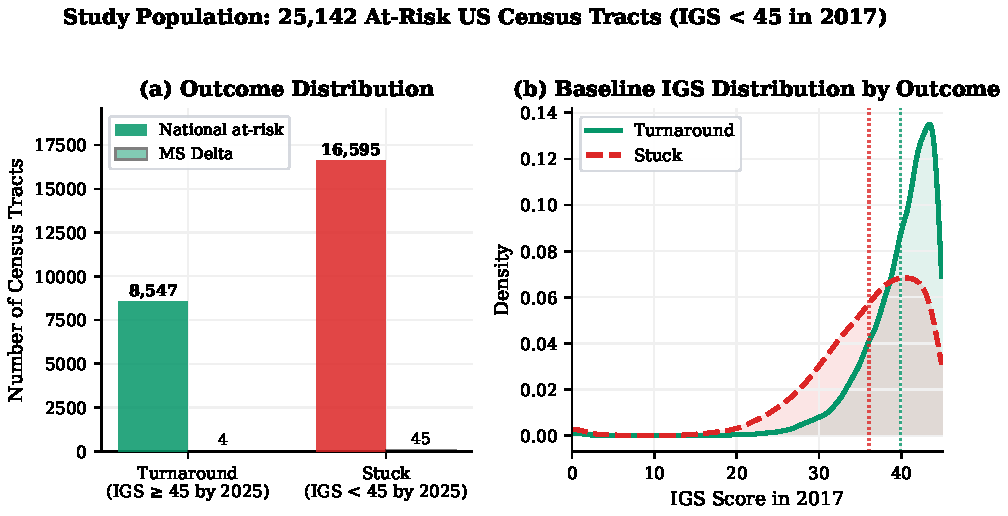
\includegraphics[width=\linewidth]{figures/fig2_study_population.pdf}
  \caption{Study population.  \textbf{(a)} Turnaround vs.\ Stuck
    counts nationally and in the MS Delta.  \textbf{(b)} Distribution
    of baseline IGS scores (2017) by outcome, showing that stuck and
    turnaround tracts share nearly identical starting conditions—the
    divergence is driven by other factors.}
  \label{fig:population}
\end{figure}

Panel~(b) of Figure~\ref{fig:population} highlights a crucial point:
turnaround and stuck tracts have almost identical baseline IGS
distributions.  The outcome is therefore not predetermined by the
starting score—it is driven by the 89 features we describe next.

\subsection{Feature Engineering}

\begin{tikzpicture}[
    node distance = 0.55cm and 1.1cm,
    box/.style    = {rectangle, rounded corners=3pt, draw=mcblue!60,
                     fill=mcblue!6, text width=2.9cm,
                     align=center, font=\small, inner sep=5pt},
    arrow/.style  = {-Stealth, thick, color=mcblue!70},
    label/.style  = {font=\footnotesize\itshape, text=midgray},
]

\node[box] (src) {10 Public\\Datasets};
\node[box, right=of src] (eng) {Feature\\Engineering\\(89 features)};
\node[box, right=of eng] (ml)  {3-Model\\Ensemble\\LR · RF · GBM};
\node[box, right=of ml]  (shp) {TreeSHAP\\(RF, 5k tracts)};

\node[box, below=0.7cm of shp] (pm) {Priority\\Matrix\\(per county)};
\node[box, below=0.7cm of eng] (gap){Gap\\Analysis};

\draw[arrow] (src) -- (eng);
\draw[arrow] (eng) -- (ml);
\draw[arrow] (ml)  -- (shp);
\draw[arrow] (shp) -- (pm);
\draw[arrow] (shp) -- (gap);
\draw[arrow] (gap) -- (pm);

\node[label, above=0.1cm of src] {Ingest};
\node[label, above=0.1cm of eng] {Build};
\node[label, above=0.1cm of ml]  {Train};
\node[label, above=0.1cm of shp] {Explain};
\end{tikzpicture}
\vspace{6pt}

We engineer \textbf{89 features} across 11 domain categories from ten
public datasets: Mastercard IGS sub-indicators (2017 baseline),
CDC~PLACES health prevalence rates, CDC~SVI granular population
percentages (replacing the four opaque RPL\_THEME composites with 13
normalized rates), USDA Food Access Atlas, County Business Patterns,
FEMA National Risk Index, CDC Environmental Justice Index, HRSA
shortage-area designations, Area Health Resources File, and SBA
lending rankings.  Every feature carries an explicit
\texttt{higher\_is\_better} flag used to orient gap directions
consistently.

\subsection{Machine-Learning Pipeline}

Three classifiers are trained using 5-fold stratified
cross-validation: \textbf{Logistic Regression} (L2 penalty, scaled
features), \textbf{Random Forest} (500 trees, balanced class weights),
and \textbf{Gradient Boosting} (histogram-based).
Table~\ref{tab:model} reports held-out ROC-AUC.

\begin{table}[h]
  \centering
  \small
  \caption{Model performance — 5-fold stratified cross-validation
    on 25,142 at-risk tracts.}
  \label{tab:model}
  \begin{tabular}{lcc}
    \toprule
    Model               & CV ROC-AUC    & Role \\
    \midrule
    Logistic Regression & 0.718 ± 0.006 & Linear baseline \\
    Random Forest       & 0.763 ± 0.005 & \shap{} source (TreeSHAP) \\
    Gradient Boosting   & 0.771 ± 0.004 & Sequential learning \\
    \bottomrule
  \end{tabular}
\end{table}

\noindent TreeSHAP is applied to the Random Forest on a random sample
of 5,000 tracts (\texttt{random\_state=42}), yielding per-tract
per-feature contributions that are additive and consistent with the
model's predictions.

% ─────────────────────────────────────────────────────────────
\section{Results}
% ─────────────────────────────────────────────────────────────

\subsection{What Drives Turnaround? (SHAP Feature Importance)}

Figure~\ref{fig:shap} shows the top 20 predictors ranked by mean
$|\text{SHAP}|$ as a share of total predictive power.  Three findings
stand out:

\begin{enumerate}[leftmargin=*, itemsep=2pt]
  \item \textbf{Preventive dental care} (\emph{Dental Visit Rate},
    9.2\%) is the single strongest predictor—stronger than any
    economic or housing feature.  The CDC~PLACES dental-visit rate
    measures the share of adults who visited a dentist or dental clinic
    in the past year (higher = better).  Turnaround tracts average
    56.9\%; the MS Delta averages only 6.1\%—a 50.8-point gap placing
    the Delta at the \textbf{1st percentile nationally}.  The SHAP
    relationship is monotonically positive (Spearman $\rho > 0$):
    every decile rise in dental-visit access pushes SHAP contributions
    toward turnaround.

  \item \textbf{Commercial diversity} (8.8\%) is the top economic
    predictor, outranking broadband access, income, and business
    counts.  A multi-sector local economy signals resilience.

  \item \textbf{Residential property values} (6.7\%) and
    \textbf{physical inactivity} (6.4\%) follow, confirming that
    health behaviors and asset endowments jointly predict recovery.
\end{enumerate}

\subsection*{Why Dental Access? A Proxy for Economic Connectivity}

The dental finding is counterintuitive at first glance but robust
across multiple validation approaches.  We propose four reinforcing
mechanisms:

\begin{enumerate}[leftmargin=*, itemsep=2pt, label=\alph*.]
  \item \textbf{Economic connectivity proxy.}  Dental-visit rate
    correlates strongly with Internet Access Score ($r = 0.469$).
    Both measure whether households are embedded in a functioning
    service economy—broadband at home and a nearby dental provider
    are co-produced by the same infrastructure and income conditions.

  \item \textbf{Healthcare system engagement.}  Preventive dental
    visits require stable transportation, health-seeking behavior,
    insurance coverage, and provider supply.  Communities where
    most adults navigate this system have already solved coordination
    problems that block recovery more broadly.  All nine Delta
    counties are 100\% designated as Primary Care Health Professional
    Shortage Areas (HPSAs), reflecting how completely the healthcare
    infrastructure has collapsed in the region.

  \item \textbf{Workforce productivity.}  Untreated dental disease
    is a well-documented cause of absenteeism and presenteeism.
    Low dental-visit rates therefore predict lower effective labor
    supply in the following year—a direct drag on economic output.

  \item \textbf{Income and insurance signal.}  Regular dental visits
    proxy for employer-sponsored insurance and sufficient disposable
    income.  A community with high dental access has a more stable
    earnings base, reducing sensitivity to local shocks.
\end{enumerate}

\noindent The implication is precise: closing the dental-access gap
in the Delta is not a ``health'' intervention in isolation—it is an
\emph{economic infrastructure} intervention that simultaneously
addresses workforce productivity, healthcare engagement, and the
proxy conditions that underpin commercial-ecosystem growth.

\begin{figure}[ht]
  \centering
  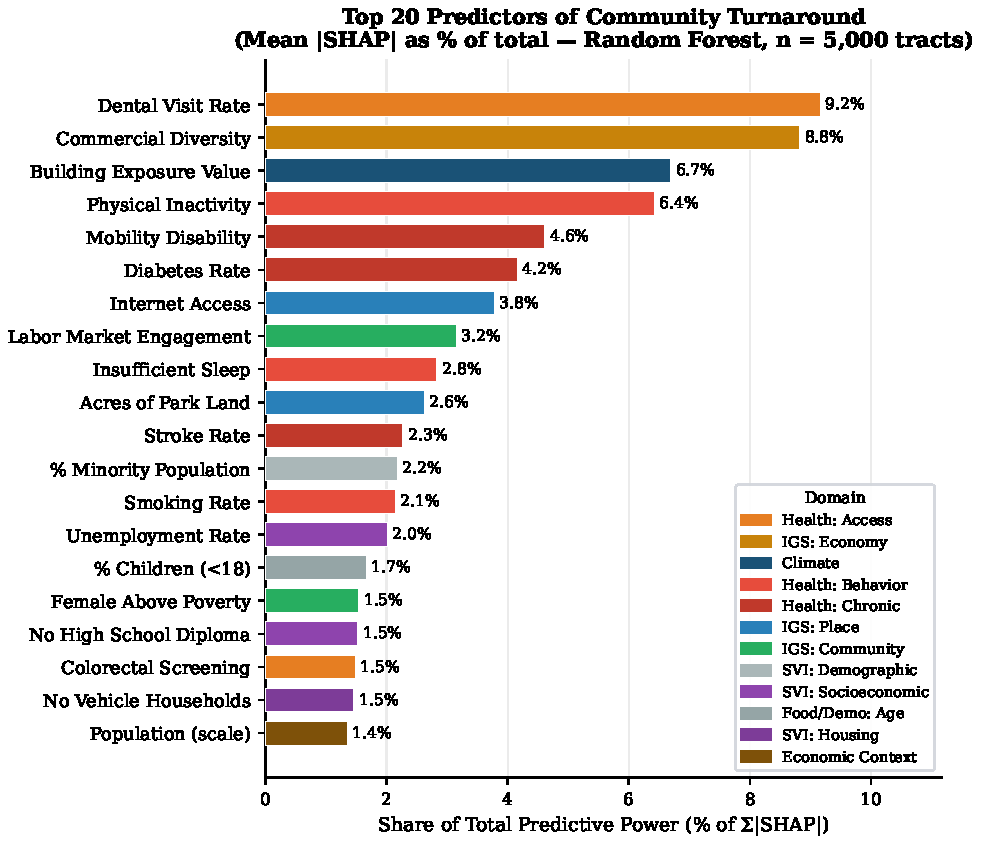
\includegraphics[width=\linewidth]{figures/fig3_shap_importance.pdf}
  \caption{Top 20 predictors of community turnaround by
    mean $|\shap{}|$ share of total predictive power.  Bar color
    indicates feature domain.  Dental-visit rates, commercial
    diversity, and property values collectively account for
    \textasciitilde{}25\% of the model's explanatory power.}
  \label{fig:shap}
\end{figure}

\subsection{Directionality — SHAP Beeswarm}

Figure~\ref{fig:beeswarm} shows the beeswarm plot for the top 15
features.  Each dot is one census tract; horizontal position is the
SHAP contribution; color encodes the feature value on a
High~(\textcolor{deltared}{$\bullet$}) to
Low~(\textcolor{mcblue}{$\bullet$}) scale.

Key patterns:
\begin{itemize}[leftmargin=*, itemsep=2pt]
  \item \emph{Dental Visit Rate}: red dots cluster right (high dental
    access $\rightarrow$ turnaround), blue dots cluster left (low
    access $\rightarrow$ stuck).  Strong, monotone positive effect.

  \item \emph{Physical Inactivity}: opposite pattern—red (high
    inactivity) clusters left, confirming it is a burden.

  \item \emph{Commercial Diversity Score}: wide spread, indicating
    tracts vary substantially in how this predictor affects their
    trajectory.
\end{itemize}

\begin{figure}[ht]
  \centering
  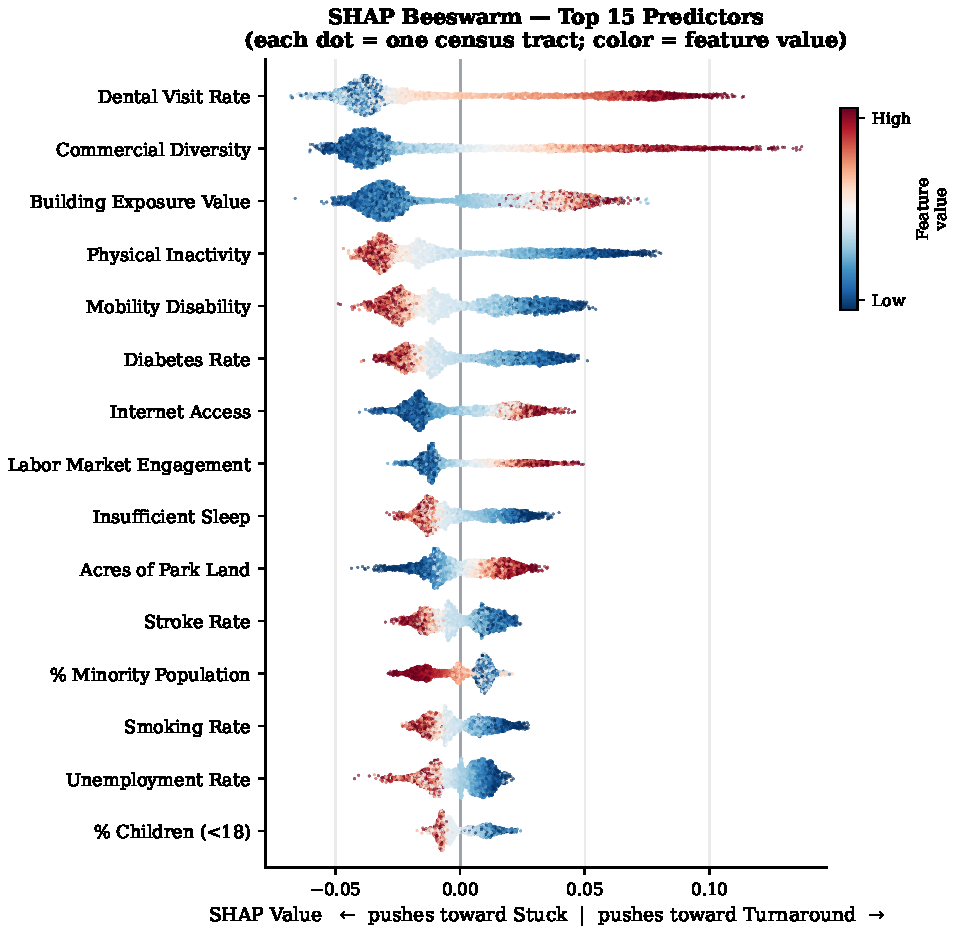
\includegraphics[width=\linewidth]{figures/fig4_beeswarm.pdf}
  \caption{\shap{} beeswarm plot for the top 15 predictors.
    Horizontal axis: SHAP value contribution (positive = pushes toward
    turnaround). Dot color: feature value
    (\textcolor{deltared}{red} = high, \textcolor{mcblue}{blue} = low).
    Density-aware vertical jitter ensures no overplotting.}
  \label{fig:beeswarm}
\end{figure}

\subsection{Domain-Level Analysis}

Figure~\ref{fig:cat} decomposes predictive power and Delta gaps by
feature domain.  Health Outcomes and IGS sub-indicators together
account for nearly half of all \shap{} importance.  The right panel
confirms that the Delta lags most severely on Health Outcomes and
Business Infrastructure—exactly the domains most predictive of
recovery.

\begin{figure}[ht]
  \centering
  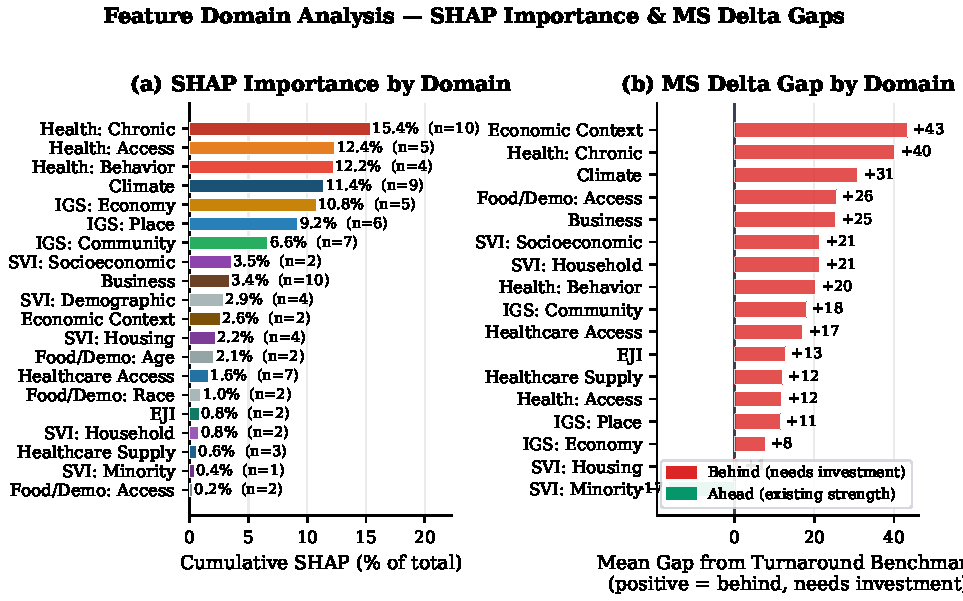
\includegraphics[width=\linewidth]{figures/fig6_category_and_gap.pdf}
  \caption{\textbf{(a)} Cumulative \shap{} importance by feature
    domain.  \textbf{(b)} Mean gap from the turnaround benchmark for
    each domain in the MS Delta (\textcolor{deltared}{red} = behind,
    \textcolor{turngreen}{green} = ahead).  The Delta's largest deficits
    are in the domains that matter most.}
  \label{fig:cat}
\end{figure}

% ─────────────────────────────────────────────────────────────
\section{Case Study: The Mississippi Delta}
% ─────────────────────────────────────────────────────────────

The Mississippi Delta is one of the most persistently distressed
regions in the United States.  All nine counties remain below IGS~45,
and the Delta's turnaround rate (24\%, vs.\ 34\% nationally) is
substantially lower than the national baseline.

\subsection{Investment Priority Matrix}

The Priority Matrix (Figure~\ref{fig:matrix}) places every feature on
two axes simultaneously: \textbf{SHAP importance} (national,
fixed—how much the model relies on this predictor globally) and
\textbf{gap from the turnaround benchmark} (Delta-specific—how far
behind the Delta lags).  This creates four actionable quadrants:

\begin{center}
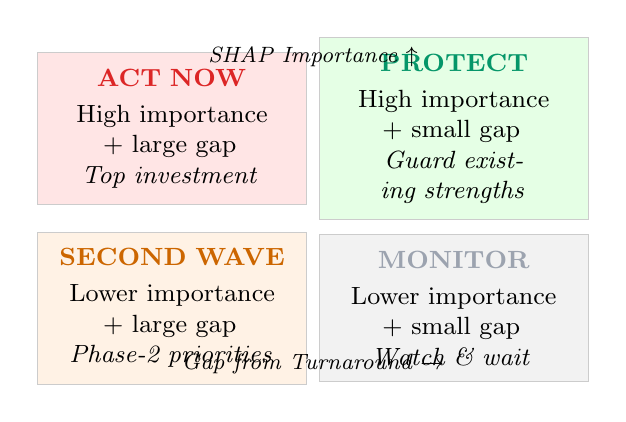
\begin{tikzpicture}[
    cell/.style={rectangle, draw=gray!40, fill=#1, text width=3.0cm,
                 align=center, inner sep=6pt, font=\small},
    label/.style={font=\footnotesize\bfseries, color=#1},
]
\matrix[column sep=4pt, row sep=4pt] {
  \node[cell=red!10]
    {\textcolor{deltared}{\textbf{ACT NOW}}\\[2pt]
     High importance\\+ large gap\\
     \textit{Top investment}};
  &
  \node[cell=green!10]
    {\textcolor{turngreen}{\textbf{PROTECT}}\\[2pt]
     High importance\\+ small gap\\
     \textit{Guard existing strengths}};
  \\
  \node[cell=orange!10]
    {\textcolor{orange!80!black}{\textbf{SECOND WAVE}}\\[2pt]
     Lower importance\\+ large gap\\
     \textit{Phase-2 priorities}};
  &
  \node[cell=gray!10]
    {\textcolor{midgray}{\textbf{MONITOR}}\\[2pt]
     Lower importance\\+ small gap\\
     \textit{Watch \& wait}};
  \\
};
\node[above=0.15cm, font=\footnotesize\itshape] at (0, 1.55)
  {SHAP Importance $\uparrow$};
\node[below=0.15cm, font=\footnotesize\itshape] at (0, -1.55)
  {Gap from Turnaround $\rightarrow$};
\end{tikzpicture}
\end{center}
\vspace{4pt}

\begin{figure}[ht]
  \centering
  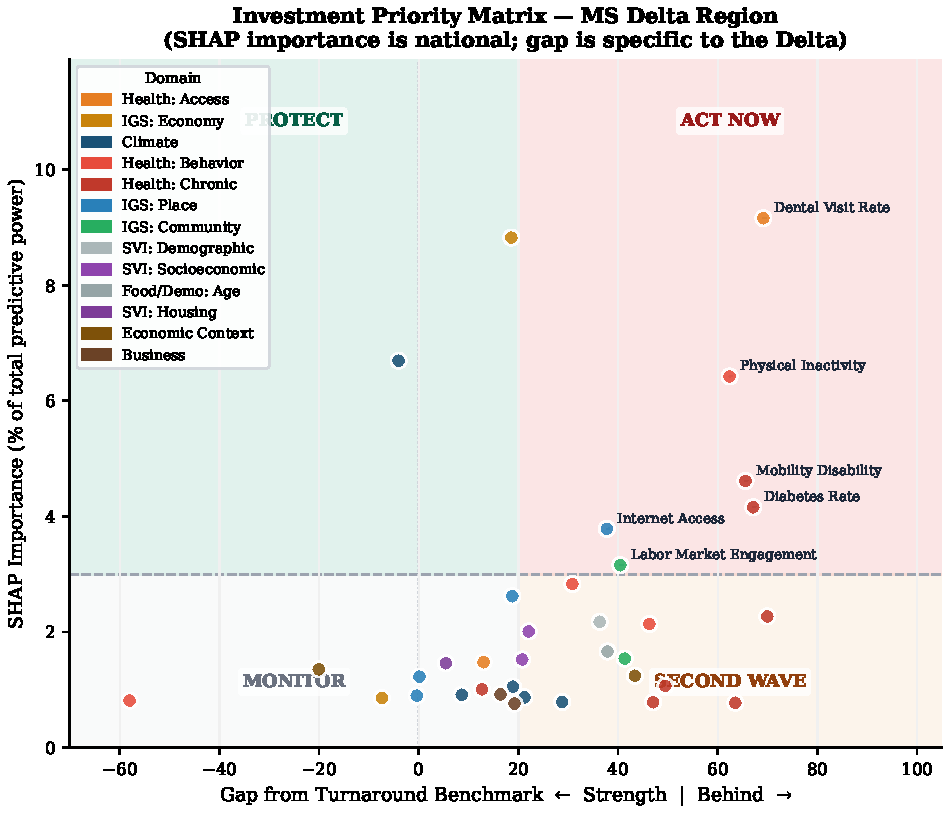
\includegraphics[width=\linewidth]{figures/fig5_priority_matrix.pdf}
  \caption{Investment Priority Matrix for the MS Delta region.
    Features in the upper-right quadrant (Act Now) are simultaneously
    the strongest national predictors \emph{and} the areas where the
    Delta is furthest behind.  Annotated labels show the most
    critical Act~Now features.}
  \label{fig:matrix}
\end{figure}

\subsection{Top Priorities for the Delta}

The Act~Now quadrant reveals a coherent intervention strategy:

\begin{itemize}[leftmargin=*, itemsep=3pt]
  \item \textbf{Preventive healthcare access} (Dental Visit Rate,
    Preventive Checkups, Colorectal Screening): The Delta's chronic
    disease burden is the #1 barrier.  FQHCs, mobile dental units,
    and Medicaid navigator programs address this directly.

  \item \textbf{Commercial ecosystem diversification} (Commercial
    Diversity Score, Food Retail): The Delta is dominated by
    mono-sector economic activity.  Small-business incubators and
    mixed-use development are the highest-ROI interventions.

  \item \textbf{Broadband connectivity} (Internet Access Score):
    Digital exclusion compounds every other gap—workforce readiness,
    telehealth access, and e-commerce all depend on reliable broadband.
\end{itemize}

The Protect quadrant identifies the Delta's existing strengths
(e.g., some housing stability metrics) that should be preserved
rather than disrupted by investment strategies.

% ─────────────────────────────────────────────────────────────
\section{Conclusion}
% ─────────────────────────────────────────────────────────────

We have shown that community economic recovery is predictable from
granular, feature-level data—and that the predictions are
\emph{interpretable} enough to drive concrete investment decisions.
The headline finding is counterintuitive: preventive dental care and
commercial diversity are stronger predictors of IGS turnaround than
broadband access, healthcare provider counts, or poverty rates.

For the Mississippi Delta, this translates to a clear priority order:
expand preventive healthcare access, diversify the commercial
ecosystem, and close the broadband gap.  Our interactive dashboard
lets county-level stakeholders explore their own Priority Matrix in
real time, updated as new IGS data becomes available.

\paragraph{Limitations.}  The turnaround definition (IGS $\geq 45$ by
2025) is a threshold outcome; continuous modeling of IGS change would
capture gradient effects.  Causal identification requires quasi-experimental
methods beyond the scope of this study.  Some features (e.g., FEMA
risk scores) are national proxies that may be imprecise at the tract
level.

\paragraph{Reproducibility.}  All code, processed data (where size
permits), and the Streamlit dashboard are available at
\href{https://github.com/SauravBhattarai19/Data_Challenge}%
{\texttt{github.com/SauravBhattarai19/Data\_Challenge}}.
The live interactive application is publicly accessible at
\href{https://howtoimprove.streamlit.app}{\texttt{howtoimprove.streamlit.app}}.

% ─────────────────────────────────────────────────────────────
\section*{Data Sources}
% ─────────────────────────────────────────────────────────────

\small
\begin{tabular}{@{}p{2.6cm}p{2.8cm}p{1.0cm}p{6.5cm}@{}}
\toprule
\textbf{Dataset} & \textbf{Producer} & \textbf{Year} & \textbf{Key variables used} \\
\midrule
Mastercard IGS &
  Mastercard Economics Institute &
  2017–25 &
  igs\_score, igs\_economy, igs\_place, igs\_community + 9 sub-indicators (tract level) \\[4pt]
CDC PLACES &
  CDC / BRFSS &
  2022 &
  27 chronic-disease prevalence rates: DENTAL, BPHIGH, OBESITY, PHLTH, CSMOKING, CHECKUP, \ldots \\[4pt]
CDC SVI &
  ATSDR &
  2022 &
  4 RPL\_THEME composite percentiles replaced by 13 normalized sub-indicator rates (poverty, disability, housing cost burden, etc.) \\[4pt]
USDA Food Atlas &
  USDA ERS &
  2019 &
  LACCESS\_POP10, PCT\_SNAP17, PCT\_NSLP17, PCT\_REDUCED\_LUNCH, food-retail access flags \\[4pt]
FEMA NRI &
  FEMA &
  2023 &
  RISK\_SCORE (composite natural hazard risk), 18 individual hazard scores \\[4pt]
CDC EJI &
  CDC ATSDR &
  2022 &
  Environmental burden index, social vulnerability, health vulnerability \\[4pt]
HRSA HPSA / MUA &
  HRSA &
  2024 &
  Primary care \& mental health HPSA scores/flags, MUA/MUP designation \\[4pt]
AHRF &
  HRSA BHPr &
  2024–25 &
  Physician, specialist, hospital counts; Medicare/Medicaid enrollment rates; county health infrastructure \\[4pt]
CBP / ZBP &
  US Census Bureau &
  2023 &
  Establishment counts by NAICS sector, employment, annual payroll (county \& ZIP) \\[4pt]
SBA Rankings &
  US Small Business Administration &
  2025 &
  State-level small-business counts, net new jobs, women-owned \%, SB employment share \\
\bottomrule
\end{tabular}
\normalsize

\end{document}
